\section{User Interface}

This section covers the principles and guideline used in order to create the \ac{GUI}.
The layout for all views, that require authorization to use, was created with the use of the Gestalt principles \citep{gestalt_principles}.
This layout is a graphical guideline, as it contains graphical elements for the \acs{GUI}, while having defined areas for dynamic content.
The reason behind using a layout is to gain similarity, as described in the Gestalt principles.
This is done to improve the user's ability to differentiate between when he or she is authorized and not authorized.

The layout used can be seen in Figure~\ref{fig:gui_layout}.
\deno{Content} of the layout is a dynamic placeholder for individual content of each view, while the menu remains the same.

\begin{figure}[htb]
    \centering
    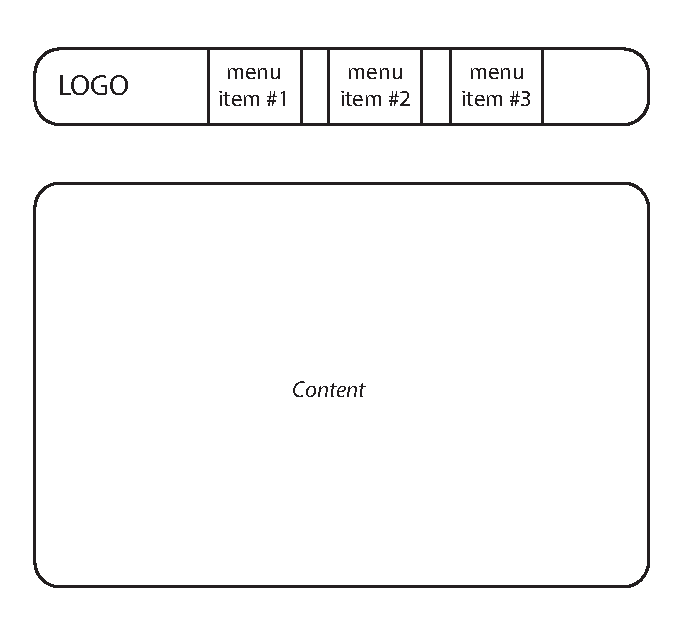
\includegraphics[width=0.8\textwidth]{gfx/gui_layout.pdf}
    \caption{\acs{GUI} layout.}
    \label{fig:gui_layout}
\end{figure}

Since the HTTP protocol is stateless and requires all parameters to be received through requests \citep{python_stateless}, it creates a behavior which might be counterintuitive to the user, e.g. when using the browser's back and forward functionality.
Moving backwards in a browsing history which involved sending parameters causes the browser to resend these parameters.
This might not be the intention of the user.
For instance, assuming a user wants to create two new roles.
The user is presented with a list of the current roles in the company, and navigates to a view allowing him to create a new role, $r_A$.
When the information about $r_A$ has been filled in, the user submits this data by creating a HTTP request to \deno{W} with parameters containing the information about $r_A$.
\deno{W} processes the parameters and creates the role $r_A$.
Then \deno{W} presents the user with a view showing $r_A$.
Assuming the user now wants to navigate back to the view of all roles via the back functionality in the browser.
The browser will perform his previous request, i.e. the request to create the role $r_A$, which \deno{W} interprets as creating a new role $r_B$ with the same parameters as $r_A$.
One way to solve this problem is to create requests in the background of the browsers history through the asynchronous requests described in Section~\ref{sec:design_client}.
